\documentclass[9pt]{article}

\usepackage[margin=2cm]{geometry}
\usepackage{hyperref}
\usepackage{algorithm}
\usepackage{algpseudocode}
\usepackage{amsmath, amsthm, amssymb}
\usepackage{multicol, multirow}
\usepackage{tikz}
\usetikzlibrary{graphs}

\newtheorem{claim}{Claim}

\title{
    \textbf{ECO311: Game Theory} \\
    \textbf{\large{Take-Home Quiz Solutions}}
}
\author{
    \href{mailto:divyajeet21529@iiitd.ac.in}{\textbf{Divyajeet Singh (2021529)}}
    \hspace*{30pt}
    \href{mailto:anoushka21133@iiitd.ac.in}{\textbf{Anoushka Kumar (2021133)}}
}
\date{}

\begin{document}
\maketitle

\section*{Solution 1.}
Given a set of 3 indivisible objects $S = \{ A, B, C \}$.

\subsection*{Part (a)}
We first model the given scenario as an extensive-form game $\Gamma = ( N, (V, E, r), \{ V_{i} \}_{i \in N}, \{ A(x) \}_{x \in V}, \{ U_{i} \}_{i \in N} )$.
The game tree is given in Figure \ref{fig:game-tree}.
\begin{figure}[htbp]
    \centering
    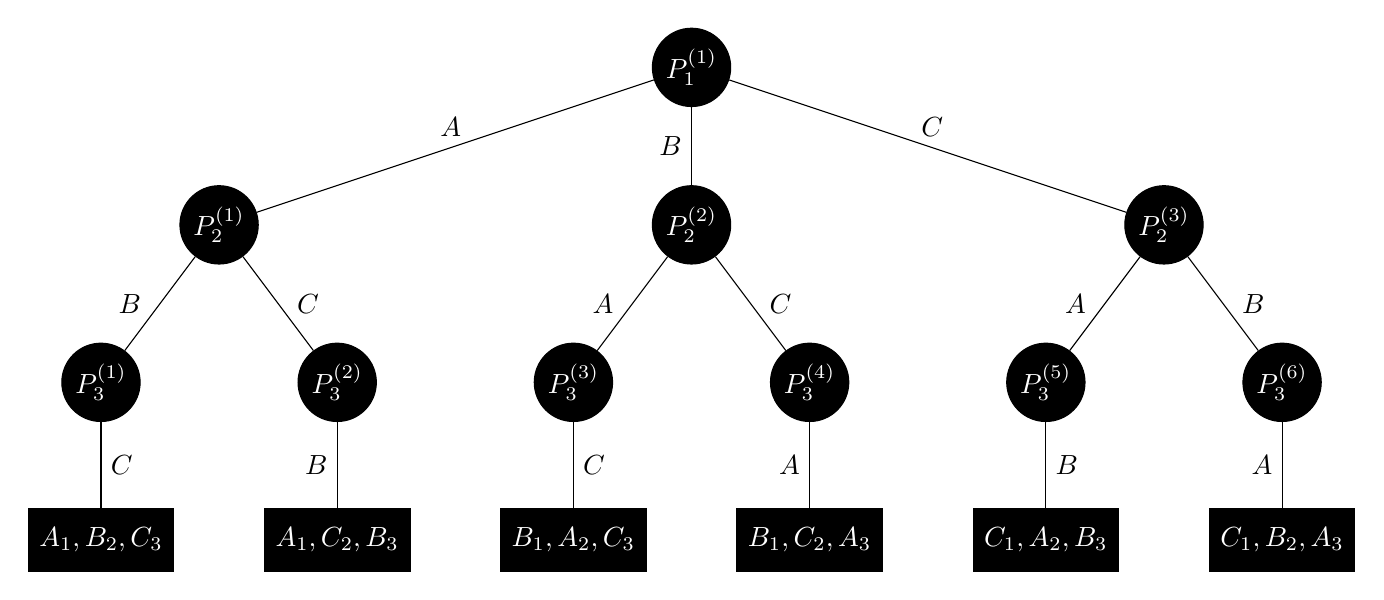
\begin{tikzpicture}[
        node rect/.style = {rectangle, draw, fill=black, text=white, inner sep=4pt, minimum width=1.2cm, minimum height=0.8cm},
        node circ/.style = {circle, draw, fill=black, text=white, inner sep=2pt},  % Style for nodes
        edge above/.style = {midway, above},
        edge left/.style = {midway, left},
        edge right/.style = {midway, right},
        ]
        \node[node circ] (P1) at (0,0) {$P_{1}^{(1)}$};

        % Level 1 nodes
        \node[node circ] (P21) at (-6, -2) {$P_{2}^{(1)}$};
        \node[node circ] (P22) at (0, -2) {$P_{2}^{(2)}$};
        \node[node circ] (P23) at (6, -2) {$P_{2}^{(3)}$};

        % Level 2 nodes
        \node[node circ] (P31) at (-7.5, -4) {$P_{3}^{(1)}$};
        \node[node circ] (P32) at (-4.5, -4) {$P_{3}^{(2)}$};
        \node[node circ] (P33) at (-1.5, -4) {$P_3^{(3)}$};
        \node[node circ] (P34) at (1.5, -4) {$P_3^{(4)}$};
        \node[node circ] (P35) at (4.5, -4) {$P_3^{(5)}$};
        \node[node circ] (P36) at (7.5, -4) {$P_3^{(6)}$};

        % Level 3 nodes
        \node[node rect] (PABC) at (-7.5, -6) {$A_{1}, B_{2}, C_{3}$};
        \node[node rect] (PACB) at (-4.5, -6) {$A_{1}, C_{2}, B_{3}$};
        \node[node rect] (PBAC) at (-1.5, -6) {$B_{1}, A_{2}, C_{3}$};
        \node[node rect] (PBCA) at (1.5, -6) {$B_{1}, C_{2}, A_{3}$};
        \node[node rect] (PCAB) at (4.5, -6) {$C_{1}, A_{2}, B_{3}$};
        \node[node rect] (PCBA) at (7.5, -6) {$C_{1}, B_{2}, A_{3}$};

        % Edges from P1 to Level 1 nodes
        \draw (P1) -- (P21) node[edge above] {$A\ $};
        \draw (P1) -- (P22) node[edge left] {$B$};
        \draw (P1) -- (P23) node[edge above] {$\ C$};

        % Edges from Level 1 to Level 2 nodes
        \draw (P21) -- (P31) node[edge left] {$B\ $};
        \draw (P21) -- (P32) node[edge right] {$\ C$};
        \draw (P22) -- (P33) node[edge left] {$A\ $};
        \draw (P22) -- (P34) node[edge right] {$\ C$};
        \draw (P23) -- (P35) node[edge left] {$A\ $};
        \draw (P23) -- (P36) node[edge right] {$\ B$};

        % Edges from Level 2 to Level 3 nodes
        \draw (P31) -- (PABC) node[edge right] {$C$};
        \draw (P32) -- (PACB) node[edge left] {$B$};
        \draw (P33) -- (PBAC) node[edge right] {$C$};
        \draw (P34) -- (PBCA) node[edge left] {$A$};
        \draw (P35) -- (PCAB) node[edge right] {$B$};
        \draw (P36) -- (PCBA) node[edge left] {$A$};
    \end{tikzpicture}
    \caption{Game tree for the given scenario.}
    \label{fig:game-tree}
\end{figure}
\vspace*{0pt} \\
where $s_{i}$ refers to the value of object $s \in S$ to player $i$.
For example, $B_{3}$ refers to the value of object $B$ to player 3.
We have the set of players $N = \{ 1, 2, 3 \}$.
Vertices $P_{i}^{(j)}$ lie in the set $V_{i}$ for each player $i \in N$.
Let $v_{i}(s)$ denote the value of object $s \in S$ to player $i \in N$.
Then, the utility $U_{i}$ for player $i$ is given by
\begin{equation}
    U_{i}(a_{1}, a_{2}, a_{3}) = v_{i}(a_{i})
\end{equation}
where $(a_{1}, a_{2}, a_{3})$ is a leaf node in the game tree.
From the game tree, we can find the set of strategies for each player.
These are
\begin{align}
    \begin{split}
        S_{1} &= \{ A, B, C \} \\
        S_{2} &= \{ BAA, BAB, BCA, BCB, CAA, CAB, CCA, CCB \} \\
        S_{3} &= \{ CCB, CCA, CAB, CAA, BCB, BCA, BAB, BAA \}
    \end{split}
\end{align}
We know that any extensive-form game can be represented as a strategic-form (matrix-form) game.
The strategic form of the game is given by the set of strategies for each player and the payoff matrix.
Using the above information, we can represent the game in strategic form by creating a $3 \times 8 \times 8$ payoff matrix.
To represent the utilities, we can draw out $3$ tables of $8 \times 8$ each, one for each possible choice of object by player 1. \\
However, we make a key observation - when player 1 and player 2 have made their choices, player 3 is forced to select the last remaining object.
This means that given any strategy of player 1 and player 2, the payoff of player 3 is fixed, i.e. the strategy of player 3 is a function of the actions taken by player 1 and player 2.
So, this is effectively a 2-player game between player 1 and player 2, based on whose choices, payoffs are generated for 3 players.
Thus, we can simplify the payoff matrix as shown in Table \ref{tab:tab3x8}.
\begin{table}[htbp]
    \centering
    \begin{tabular}{c|cccccccc}
        & $BAA$ & $BAB$ & $BCA$ & $BCB$ & $CAA$ & $CAB$ & $CCA$ & $CCB$ \\
        \hline
        $A$ & $A_{1}, B_{2}, C_{3}$ & $A_{1}, B_{2}, C_{3}$ & $A_{1}, B_{2}, C_{3}$ & $A_{1}, B_{2}, C_{3}$ & $A_{1}, C_{2}, B_{3}$ & $A_{1}, C_{2}, B_{3}$ & $A_{1}, C_{2}, B_{3}$ & $A_{1}, C_{2}, B_{3}$ \\
        $B$ & $B_{1}, A_{2}, C_{3}$ & $B_{1}, A_{2}, C_{3}$ & $B_{1}, C_{2}, A_{3}$ & $B_{1}, C_{2}, A_{3}$ & $B_{1}, A_{2}, C_{3}$ & $B_{1}, A_{2}, C_{3}$ & $B_{1}, C_{2}, A_{3}$ & $B_{1}, C_{2}, A_{3}$ \\
        $C$ & $C_{1}, A_{2}, B_{3}$ & $C_{1}, B_{2}, A_{3}$ & $C_{1}, A_{2}, B_{3}$ & $C_{1}, B_{2}, A_{3}$ & $C_{1}, A_{2}, B_{3}$ & $C_{1}, B_{2}, A_{3}$ & $C_{1}, A_{2}, B_{3}$ & $C_{1}, B_{2}, A_{3}$\\
    \end{tabular}
    \caption{Strategies of player 1 vs strategies of player 2 (payoff of player 3 gets fixed).}
    \label{tab:tab3x8}
\end{table}
\vspace*{0pt} \\
where each entry is of the form $(X_{1}, Y_{2}, Z_{3})$, denoting the payoff of player 1, player 2, and player 3 respectively on the given strategy profile.
Thus, the above payoff matrix is the strategic-form of the game.

\subsection*{Part (b)}
Yes, the game has a pure-strategy Nash equilibrium.
Define $s_{1}^{*}$, $s_{2}^{*}$, and $s_{3}^{*}$ as follows.
\begin{equation}
    s_{1}^{*} = \underset{s \in S}{\text{argmax}} \ v_{1}(s)
    \qquad
    s_{2}^{*} = \underset{s \in S \setminus \left\{ s_{1}^{*} \right\}}{\text{argmax}} \ v_{2}(s)
    \qquad
    s_{3}^{*} \in S \setminus \left\{ s_{1}^{*}, s_{2}^{*} \right\}
\end{equation}
Then, the strategy profile $\left( s_{1}^{*}, s_{2}^{*}, s_{3}^{*} \right)$ is a Nash equilibrium.
This is because player 1 gets the object of their highest preference (i.e. cannot obtain a higher payoff).
Player 2 gets the object of their highest preference among the remaining objects.
Player 3 gets the last object, which is the only one available.
Since the payoff of each object is strictly positive, player 3 still receives a positive payoff.
Thus, no player can benefit by unilateral deviation.

\subsubsection*{Deriving the equilibrium strategy profile using backward induction}
We can also derive the same strategy profile as the Nash equilibrium using backward induction as follows.
Nodes $P_{3}^{j}$ effectively make no choice and their corresponding payoffs move up the tree.
So, the action taken by player 3 can be written as
\begin{equation}
    s_{3}^{*} \in S \setminus \left\{ s_{1}^{*}, s_{2}^{*} \right\} = \begin{cases}
        C & \text{if } \{ s_{1}^{*}, s_{2}^{*} \} = \{ A, B \} \\
        B & \text{if } \{ s_{1}^{*}, s_{2}^{*} \} = \{ A, C \} \\
        A & \text{if } \{ s_{1}^{*}, s_{2}^{*} \} = \{ B, C \}
    \end{cases}
\end{equation}
where $s_{1}^{*}$ and $s_{2}^{*}$ are the actions of player 1 and player 2 respectively.
$P_{2}^{(1)}$ chooses between the payoffs $(A_{1}, B_{2}, C_{3})$ and $(A_{1}, C_{2}, B_{3})$, and chooses an action based on whether $B_{2} > C_{2}$ or vice-versa.
Similarly, the choices at nodes $P_{2}^{(2)}$ and $P_{2}^{(3)}$ is governed by whether $A_{2} > C_{2}$ and $A_{2} > B_{2}$ respectively.
Mathematically, this choice can be written as
\begin{equation}
    s_{2}^{*} = \underset{s \in S \setminus \left\{ s_{1}^{*} \right\}}{\text{argmax}} \ v_{2}(s)
    = \begin{cases}
        \begin{cases}
            B & \text{if } v_{2}(B) > v_{2}(C) \\
            C & \text{otherwise} \\
        \end{cases} & \text{if } s_{1}^{*} = A
        \vspace*{7pt} \\
        \begin{cases}
            A & \text{if } v_{2}(A) > v_{2}(C) \\
            C & \text{otherwise} \\
        \end{cases} & \text{if } s_{1}^{*} = B
        \vspace*{7pt} \\
        \begin{cases}
            A & \text{if } v_{2}(A) > v_{2}(B) \\
            B & \text{otherwise} \\
        \end{cases} & \text{otherwise}
    \end{cases}
\end{equation}
Finally, player 1 can choose the object of their highest preference, since $P_{2}^{(1)}$, $P_{2}^{(2)}$, and $P_{2}^{(3)}$ forward a payoff of the form $(A_{1}, s_{2}, s_{3})$, $(B_{1}, s_{2}, s_{3})$, and $(C_{1}, s_{2}, s_{3})$ to $P_{1}^{(1)}$ respectively.
Thus, the action taken by player 1 is
\begin{equation}
    s_{1}^{*} = \underset{s \in S}{\text{argmax}} \ v_{1}(s)
    = \begin{cases}
        A & \text{if } v_{1}(A) > v_{1}(B) \text{ and } v_{1}(A) > v_{1}(C) \\
        B & \text{if } v_{1}(B) > v_{1}(A) \text{ and } v_{1}(B) > v_{1}(C) \\
        C & \text{otherwise}
    \end{cases}
\end{equation}
Thus, the Nash equilibrium strategy profile obtained by backward induction is the same, i.e. $(s_{1}^{*}, s_{2}^{*}, s_{3}^{*})$.

\subsection*{Part (c)}
Now, after the game, each player is asked to state whether they are happy with their allocation or want to exchange it with another player.
If any player says that they want to exchange, then every player receives 0 payoff. \\
We make a few standard assumptions:
\begin{itemize}
    \item \textbf{Principle of Individual Rationality:} The players are perfectly rational, and aim to maximize their payoff.
    \item \textbf{Principle of Common Knowledge:} The players know that all other players are rational.
    \item Players are aware that asking for an exchange results in a 0 payoff for them (and all other players).
\end{itemize}
Then, we can assume that being `\textit{happy}' simply means whether a player has a non-zero payoff.
Each object yields a strictly positive payoff to each player.
So, even if a player receives an object not of their highest preference, they are better off `lying' that they are \textit{happy} with the allocation, since asking for an exchange would result in a 0 payoff.
Thus, all (rational) players say that they are \textit{happy} with the allocation (even if they are not!).
Consequently, the Nash equilibrium $(s_{1}^{*}, s_{2}^{*}, s_{3}^{*})$ remains unchanged. \\

\section*{Solution 2.}
Let us denote the set of players by $N = \{ B, S \}$, where $B$ is the buyer and $S$ is the seller.
$B$ believes that the car is of high quality ($H$) with probability 0.4 and of low quality ($L$) with probability 0.6.
Let $p$ be the price at which the car is sold.
Table \ref{tab:payoff-low} and Table \ref{tab:payoff-high} show the payoffs of the buyer and seller for the low-quality and high-quality car respectively.
\begin{table}[htbp]
    \centering
    \begin{tabular}{c|cc}
        & $p = 0$ & $p = 1$ \\
        \hline
        $B$ & 0 & 1 \\
        $S$ & 1 & 0 \\
    \end{tabular}
    \caption{Payoff matrix for the low-quality car.}
    \label{tab:payoff-low}
\end{table}

\section*{Solution 3.}
Given that in a zero-sum game, $(\sigma_{1}, \sigma_{2})$ and $(\sigma_{1}', \sigma_{2}')$ are two mixed-strategy nash equilibria.
Let $A_{1}$ and $A_{2}$ be the action sets of players $P_{1}$ and $P_{2}$ respectively.
Then, let $U_{1}(\alpha, \beta) = U(\alpha, \beta)$ denote the expected utility of $P_{1}$ when $P_{1}$ plays mixed strategy $\alpha \in \Delta A_{1}$ and $P_{2}$ plays mixed strategy $\beta \in \Delta A_{2}$.
Consequently, $U_{2}(\alpha, \beta) = -U(\alpha, \beta)$ is the expected utility of $P_{2}$ on the same strategy profile, since the game is zero-sum. \\
Let $(\rho_{1}, \rho_{2})$ be a mixed-strategy nash equilibrium.
Then,
\begin{align}
    \begin{split}
        U_{1}(\rho_{1}, \rho_{2}) \geq U_{1}(\alpha, \rho_{2})
        \implies U(\alpha, \rho_{2}) \leq U(\rho_{1}, \rho_{2})
    \end{split}
\end{align}
holds for any $\alpha \in \Delta A_{1}$.
Similarly, for any $\beta \in \Delta A_{2}$,
\begin{align}
    \begin{split}
        U_{2}(\rho_{1}, \rho_{2}) \geq U_{2}(\rho_{1}, \beta)
        \implies -U(\rho_{1}, \rho_{2}) \geq -U(\rho_{1}, \beta)
        \implies U(\rho_{1}, \rho_{2}) \leq U(\rho_{1}, \beta)
    \end{split}
\end{align}
Therefore, for any MSNE $(\rho_{1}, \rho_{2})$, we have, for every $\alpha \in \Delta A_{1}$ and $\beta \in \Delta A_{2}$,
\begin{equation}
    U(\alpha, \rho_{2}) \leq U(\rho_{1}, \rho_{2}) \leq U(\rho_{1}, \beta)
\end{equation}
Since $(\sigma_{1}, \sigma_{2})$ and $(\sigma_{1}', \sigma_{2}')$ are two mixed-strategy nash equilibria, we have, for every $\alpha \in \Delta A_{1}$ and $\beta \in \Delta A_{2}$,
\begin{align}
    \label{eq:msne-1}
    U(\alpha, \sigma_{2}) &\leq U(\sigma_{1}, \sigma_{2}) \leq U(\sigma_{1}, \beta) \\
    \label{eq:msne-2}
    U(\alpha, \sigma_{2}') &\leq U(\sigma_{1}', \sigma_{2}') \leq U(\sigma_{1}', \beta)
\end{align}
Substitute $\alpha = \sigma_{1}'$ and $\beta = \sigma_{2}'$ in \eqref{eq:msne-1} and $\alpha = \sigma_{1}$ and $\beta = \sigma_{2}$ in \eqref{eq:msne-2}.
This yields
\begin{equation}
    U(\sigma_{1}', \sigma_{2}) \leq U(\sigma_{1}, \sigma_{2}) \leq U(\sigma_{1}, \sigma_{2}')
    \leq U(\sigma_{1}', \sigma_{2}') \leq U(\sigma_{1}', \sigma_{2})
\end{equation}
Since the left-hand and right-hand side of the inequality are equal, the inequalities appear as strict equalities.
Thus, we have
\begin{equation}
    U(\sigma_{1}, \sigma_{2}) = U(\sigma_{1}, \sigma_{2}') = U(\sigma_{1}', \sigma_{2}) = U(\sigma_{1}', \sigma_{2}')
\end{equation}
Since all MSNE have the same expected utility in a zero-sum game, and we have shown the expected utility of the strategy profiles $(\sigma_{1}, \sigma_{2}')$ and $(\sigma_{1}', \sigma_{2})$ to be equal to the expected utility of the MSNE, we are done.
In other words,
\begin{align}
    U(\alpha, \sigma_{2}') &\leq U(\sigma_{1}', \sigma_{2}') = U(\sigma_{1}, \sigma_{2}') \leq U(\sigma_{1}, \beta) \\
    U(\alpha, \sigma_{2}) &\leq U(\sigma_{1}, \sigma_{2}) = U(\sigma_{1}', \sigma_{2}) \leq U(\sigma_{1}', \beta)
\end{align}
holds for every $\alpha \in \Delta A_{1}$ and $\beta \in \Delta A_{2}$, which are the conditions for MSNE.

\end{document}